\documentclass{article}[11pt]
\usepackage{Geoff,graphicx,subcaption}

% Please attach a 3-page detailed description of your thesis research in the US, including your project in France. As a general guide, we suggest using Times New Roman, Arial or Calibri fonts, size 11 or larger with 1 inch margins. If you can include citations in the 3 pages, please do so, but you may also add an additional page for citations. You may submit 1 file.

\begin{document}
\title{\vspace{-3cm}Advanced Multimodal Information Processing\vspace{-0.3cm}}
\author{Geoffrey Iyer} \date{}

\maketitle

\section{Introduction}
\label{sec:intro}

With the increasing availibility of data we often come upon multiple datasets,
derived from different sensors, that describe the same object or phenomenon. We
call the sensors \emph{modalities}, and because each modality represents some
new information, it is generally desirable to use more modalities rather than
fewer. For example, in the area of speech recognition, researchers have found
that integrating the audio data with a video of the speaker results in a much
more accurate classification \cite{Potamianos03,
  sedighin:hal-01400542}. Similary, in medicine, the authors of \cite{Lei12} and
\cite{Samadi2016} fuse the results of two different types of brain imaging to
create a final image with better resolution than either of the
originals. However, correctly processing a multimodal dataset is not a simple
task. Even the naive method of analyzing each modality separately still requires
clever thinking when combining the results, and this is rarely the optimal way
to handle the data. Our goal is to create a general algorithm for feature
extraction and data segmentation that can be applied to any multimodal dataset.

In the current state of the project, we consider the case where each dataset
contains the same number of elements, and these elements are co-registered (so
the $i$-th point in one set corresponds to the $i$-th point in another). This is
often the case in image processing problems, where the sets may be images of the
same scene obtained from different sensors (as is the case in our experimental
data), or taken at different times. For notation, we label the sets,
$X^1,X^2,\ldots,X^k$, with dimensions $d_1,d_2,\ldots,d_k$, and let
$X = (X^1,X^2,\ldots,X^k)\subset \R^{n\times (d_1+\cdots+d_k)}$ be the
concatenated dataset. Our method extracts features from the dataset by finding
eigenvectors of the graph Laplacian, then uses standard data-segmentation
algorithms on these features to obtain a final classification.  In section
\ref{sec:method} we give the general theory behind our method, and in
\ref{sec:experiment} we show the results of the method applied to an
optical/LIDAR dataset. Finally, in section \ref{sec:future} we discuss the
extensions of the project that we hope to complete in France.

% This is an old paragraph that I replaced, but I think I want to keep the
% notation:
%%% In this paper we address the question of segmentation of multimodal
%%% datasets. We provide an unsupervised method for data classification Blah
%%% blah blah blah. Two datasets, $X^s$, $X^t$, that describe the same
%%% object. Our goal is to somehow combine the sets to form one set $Y$ that
%%% blah blah. In the general scenario, $X^s$ and $X^t$ will often contain
%%% redundant information. Previous methods attempt to correlate the redundant
%%% parts of the two sets, but this often results in a overall loss of
%%% information, as the data unique to the individual sets isn't properly
%%% considered. In this paper we aim to emphasize the nonredundant data in our
%%% creation of $Y$.  Maybe we set up some notation here.

\section{The Method}
\label{sec:method}

\subsection{The Graph Min-Cut Problem} \label{sec:GraphMinCut} We represent our
dataset $X$ as a \emph{similarity matrix}. That is, for each two data points
$x_i, x_j$, we define a \emph{weight} $w_{ij}$ representing the similarity
between the points. A large weight corresponds to very similar nodes, and a
small weight to dissimilar nodes. There are many different choices of the
weights $w_{ij}$ in the literature, and each has its own merits. In most
applications, one defines
\[w_{ij} = \text{exp}\left(-\norm{v_i -v_j} / \sigma \right),\] where $\sigma$
is a scaling parameter. In this work we adapt this definition to apply to our
multimodal dataset. First we scale our sets $X^1,\ldots, X^k$ to make distances
in each set comparable, then we define.
\[w_{ij} = \text{exp}\left(-\max\left(\norm{x_i^1 - x_j^1}, \ldots, \norm{x_i^k
        - x_j^k}\right)\right).\] Choosing to use the maximum of the individual
values allows us to take advantage of the unique information in each dataset, as
two points are only considered similar here when they are similar in every
modality.

Moving forward, we aim to find a classification that groups pairs with high
weight together, while also separating pairs with low weight.  This goal is
formalized as the Ratio Cut problem. Given a partition of $X$ into subsets
$A_1,A_2,\ldots,A_m$, we define the \emph{ratio graph-cut}
\[\text{RatioCut}(A_1,\ldots,A_m) = \sum_{i=1}^m
  \frac{W(A_i,A_i^c)}{\abs{A_i}},\] where
$W(A,B) = \sum_{i\in A, j\in B}w_{ij}.$ Minimizing the ratio cut will give the
classification we desire, as the $W(A_i,A_i^c)$ term penalizes partitions that
separate elements with a large weight between them, while the $\abs{A_i}$ term
ensures that each segment of the final partition is of a reasonable size
(without the $\abs{A_i}$ term, the optimal solution often contains one large set
and $m-1$ small sets). It has been shown in \cite{Goldschmidt94} that explicitly
solving this problem is an $O(\abs{V}^{m^2})$ process. As this is infeasible in
most cases, we instead introduce the graph Laplacian to handle an approximation
of the minimization problem.

\subsection{Graph Laplacian and Clustering} \label{subsec:graphLaplacian} In
\cite{Mohar91} it is shown that the Ratio Cut problem can be approximately
solved using the eigenvectors of the \emph{graph Laplacian}, $L = D - W$. Here
$D$ is a diagonal matrix with entries $d_{ii}=\sum_j w_{ij}$.  Each eigenvector
represents a feature of the data, and if we let $H$ be a matrix where the
columns are eigenvectors, then the $i$th row of $H$ represents the features of
the data point $x_i$. We then get an approximate solution to the original
min-cut problem by using any data clustering algorithm on these rows. In section
\ref{sec:experiment} we use $k$-means to segment the row vectors, resulting in a
well-known algorithm called \emph{spectral clustering}.

Calculating the full graph Laplacian is computationally intensive, as the matrix
contains $n^2$ entries. Instead we use Nystr\"{o}m's extension to find
approximate eigenvalues and eigenvectors with a heavily reduced computation
time. Essentially, this consists of choosing a small number $m \ll n$ of columns
of the weight matrix, and using some clever linear algebra to approximately
solve the eigenproblem using only these columns. This results in a significant
reduction in computation time, as we compute and store matrices of size at most
$m\times n$, rather than $n\times n$. See \cite{Fowlkes04}, \cite{Merkurjev13}
for a more complete discussion of this method. In practice, $m$ can be chosen to
be quite small without creating significant error. In Section
\ref{sec:experiment} we use $m = n^{\frac{1}{4}}$.

\section{Experiment}
\label{sec:experiment}

We test our algorithm on an optical/LIDAR dataset from the 2015 IEEE Data Fusion
Contest \cite{7536139}. The data consists of an RBG image and an elevation map
of a residential neighborhood in Belgium. Each picture contains roughly 160,000
pixels.

\begin{figure}[htb]

  
\begin{subfigure}{.33\textwidth}
  \centering
  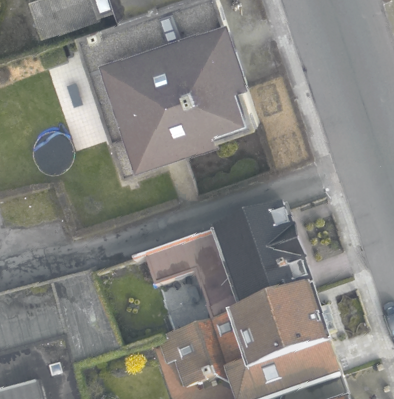
\includegraphics[width=.8\linewidth]{./Images/DFC2015/optical.png}
  \caption{Original optical data}
  \label{fig:optical}
\end{subfigure}%
\begin{subfigure}{.33\textwidth}
  \centering
  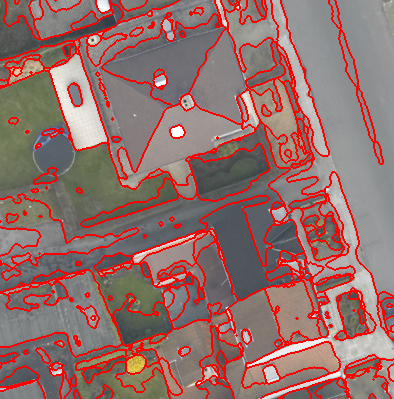
\includegraphics[width=.8\linewidth]{./Images/DFC2015/opticalOnly.png}
  \caption{Optical-only classification}
  \label{fig:opticalOnly}
\end{subfigure}
\begin{subfigure}{.33\textwidth}
  \centering
  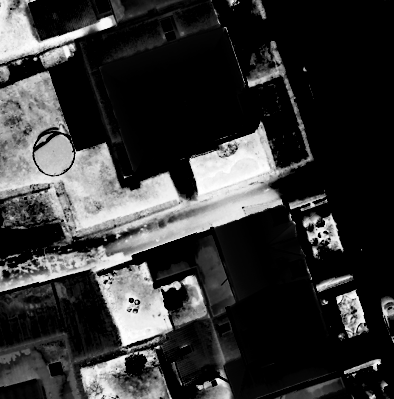
\includegraphics[width=.8\linewidth]{./Images/DFC2015/evec2.png}
  \caption{Example eigenvector}
  \label{fig:evec}
\end{subfigure}
\begin{subfigure}{.33\textwidth}
  \centering
  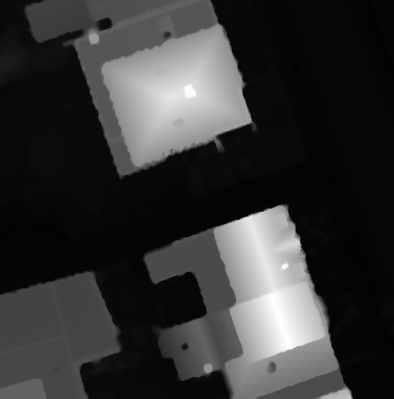
\includegraphics[width=.8\linewidth]{./Images/DFC2015/lidar.png}
  \caption{Original lidar data}
  \label{fig:lidar}
\end{subfigure}
\begin{subfigure}{.33\textwidth}
  \centering
  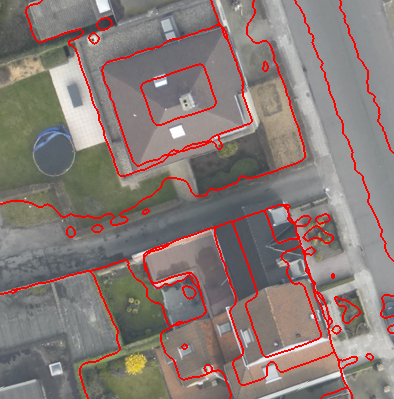
\includegraphics[width=.8\linewidth]{./Images/DFC2015/lidarOnly.png}
  \caption{Lidar-only classification}
  \label{fig:lidarOnly}
\end{subfigure}
\begin{subfigure}{.33\textwidth}
  \centering
  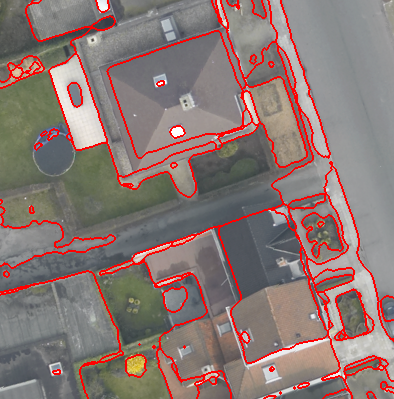
\includegraphics[width=.8\linewidth]{./Images/DFC2015/withBorders.png}
  \caption{Our classification}
  \label{fig:classification}
\end{subfigure}
\caption{Experimental results}
\label{fig:experiment}
\end{figure}

In figure \ref{fig:opticalOnly} and \ref{fig:lidarOnly} we show the results of
spectral clustering applied to each dataset individually, and the final results
of our algorithm are pictured in \ref{fig:classification}. These images show the
importance of the multimodal approach, as the optical-only method is unable to
differentiate the dark-grey roof from the adjacent street, and the lidar-only
method cannot separate the white sidewalk from the green grass. In figure
\ref{fig:evec} we show an example eigenvector of the graph Laplacian. As
explained in \ref{subsec:graphLaplacian}, this eigenvector represents one
feature extracted from our dataset. Notice how the dark-grey street is
highlighted, while both the light-grey sidewalk (which is at the same elevation)
and the nearby roof (which is the same color) are blacked out. This shows at the
level of the feature vectors that our algorithm is successfully using both the
optical and the lidar data when determining what pixels can be considered
similar. The grayscale difference in the example feature vector then causes the
classification algorithm to separate those regions in the final result
\ref{fig:classification}.

\section{Future Work}
\label{sec:future}

Our current algorithm allows us to perform feature extraction and data
segmentation on multimodal sets, as desired, but the assumption that the
datasets are \emph{co-registered} is quite restrictive. In section
\ref{sec:experiment} our two images are of the same underlying scene, where
pixels correspond exactly between images. We could not, for example, process two
images taken from different angles. Our goal for the future is to remove this
restriction and develop an algorithm that can be applied to a much larger
variety of datasets.

We approach this problem through the viewpoint of manifold alignment. Assuming
that each dataset originates from some underlying manifold, we can compare the
topologies of the different manifolds to obtain some information about the
underlying source object. Often this is done by mapping each dataset into one
common \emph{latent space}, then analyzing this amalgam of data. The major
obstacle to overcome is the inherent loss of information that comes with
transferring the original data to the latent space. This technique has been used
in \cite{Yang13,Wang11,Yeh14}, but for different purposes. These authors align
the manifolds in order to take learning accomplished on one set and transfer it
to another. Unforunately, these techniques will not directly solve our problem,
since we specifically look to perform our analysis using each modality
simultaneously, rather than working with the sets as individuals. Each modality
has its own unique advantages and disadvantages, and a transfer of learned
information implies that we ignore entirely the unique information found in the
target set. Similar to our experiment in \ref{sec:experiment}, we should expect
to better feature extraction and segmentation results when using the datasets in
tandem.  Still, the underlying idea of looking at correlations between data
points and using this to create a latent space serves as a good starting point
for our research. So, moving forward, we aim to adapt these manifold alignment
techniques to create a latent space that takes into account the
information from each modality.

We are especially excited to continue this work in France, as it would give us
the opportunity to collaborate with Christian Jutten of the GIPSA Lab in
Grenoble. Jutten is an expert in multimodal data fusion
\cite{lahat:hal-01062366}, as well as the principal investigator in the CHESS
(Challenges in extraction and separation of sources) group, which deals with
multimodal source separation. This corresponds well to our research plan, as
source separation is often the same thing as data classification. For example,
in \cite{sedighin:hal-01400542} they were able to use audio and visual
information to successfully separate different human voice signals. Also, they
developed a new approach to perform independent component analysis
simultaneously over multiple datasets \cite{lahat:hal-01351209}. These kinds of
advances all require correlating information across multiple modalities, which
is exactly the topic of our research.


\bibliographystyle{unsrt} \bibliography{../BibTex/research}

\end{document}
